\documentclass[11pt,a4paper]{article}
\usepackage[brazil]{babel}
\usepackage[utf8]{inputenc}
\usepackage[T1]{fontenc}

\usepackage{graphicx}



\begin{document}
\title{Implementação e Avaliação do Processador "FEMTOMIPS"}
\author{PCS 2405 \\ Adriano Dennani \\ Ian Elmôr Lang \\ João Henrique Kersul Faria \\ Mateus Fonseca}
\date{Julho de 2016}
\maketitle
\tableofcontents

\graphicspath{ {diagramas/} }

\section{Introdução}

\subsection{Arquitetura conjunto de instruções}

\begin{table}[]
\centering
\caption{My caption}
\label{my-label}
\begin{tabular}{|l|l|l|l|l|l|}
\hline
\textbf{31$\sim$26}      & \textbf{25$\sim$21}     & \textbf{20$\sim$16}     & \textbf{15$\sim$11}     & \textbf{10$\sim$06}        & \textbf{05$\sim$00}       \\ \hline
\multicolumn{1}{|c|}{Op} & \multicolumn{1}{c|}{Rs} & \multicolumn{1}{c|}{Rt} & \multicolumn{1}{c|}{Rd} & \multicolumn{1}{c|}{Shamt} & \multicolumn{1}{c|}{Func} \\ \hline
\end{tabular}
\end{table}

\begin{table}[]
\centering
\caption{Instruções Lógico Aritméticas}
\label{my-label}
\begin{tabular}{|l|l|l|l|}
\hline
              & \textbf{op} & \textbf{funct} & \textbf{operação}                                                                                                             \\ \hline
\textbf{add}  & 0x00        & 0x20           & GPR{[}rd{]} \textless= signed(GRP{[}rs{]}) + signed(GPR{[}rt{]})                                                              \\ \hline
\textbf{slt}  & 0x00        & 0x1A           & \begin{tabular}[c]{@{}l@{}}Se (GPR{[}rs{]} \textless GPR{[}rt{]}) então GPR{[}rd{]} = 1 se\\ não GPR{[}rd{]} = 0\end{tabular} \\ \hline
\textbf{jr}   & 0x00        & 0x08           & PC \textless= GPR{[}rs{]}                                                                                                     \\ \hline
\textbf{addu} & 0x00        & 0x21           & GPR{[}rd{]} \textless= unsigned(GRP{[}rs{]}) + unsigned(GPR{[}rt{]})                                                          \\ \hline
\textbf{sll}  & 0x00        & 0x00           & GPR{[}rd{]} \textless= GPR{[}rt{]} \textless\textless shamt                                                                   \\ \hline
\end{tabular}
\end{table}

\begin{table}[]
\centering
\caption{My caption}
\label{my-label}
\begin{tabular}{|c|c|c|c|}
\hline
\textbf{31$\sim$26} & \textbf{25$\sim$21} & \textbf{20$\sim$16} & \textbf{15$\sim$00}   \\ \hline
Op                  & Rs                  & Rt                  & Endereço/Deslocamento \\ \hline
\end{tabular}
\end{table}

\begin{table}[]
\centering
\caption{Instruções com campo imediato}
\label{my-label}
\begin{tabular}{|l|l|l|}
\hline
              & \textbf{op} & \textbf{operação}                                                                                                      \\ \hline
\textbf{lw}   & 0x23           & GPR{[}rt{]} = Mem{[}GPR{[}rs{]} + Desl{]}                                                                              \\ \hline
\textbf{sw}   & 0x2B           & Mem{[}GPR{[}rt{]}+Desl{]} = GPR{[}rs{]}                                                                                \\ \hline
\textbf{addi} & 0x08           & GPR{[}rt{]} = GPR{[}rs{]} + Imed                                                                                       \\ \hline
\textbf{beq}  & 0x04           & Se GPR{[}rs{]} = GPR{[}rt{]} então PC = PC + 4*Desl                                                                    \\ \hline
\textbf{bne}  & 0x05           & Se GPR{[}rs{]} != GPR{[}rt{]} então PC = PC + 4*Desl                                                                    \\ \hline
\textbf{slti} & 0x0A           & \begin{tabular}[c]{@{}l@{}}Se (GPR{[}rs{]} \textless Imed) então GPR{[}rt{]} = 1 se\\ não GPR{[}rt{]} = 0\end{tabular} \\ \hline
\end{tabular}
\end{table}

\begin{table}[]
\centering
\caption{Instruções de desvio Incondicional}
\label{my-label}
\begin{tabular}{|l|l|l|}
\hline
             & \textbf{op} & \textbf{operação}                           \\ \hline
\textbf{j}   & 0x02        & PC = PC(31:28) \& (4*Desl)                  \\ \hline
\textbf{jal} & 0x03        & GPR{[}7{]} = PC; PC = PC(31:28) \& (4*Desl) \\ \hline
\end{tabular}
\end{table}
	
\subsection{Visão geral do Projeto}

	Elabora-se a seguir uma visão de alto nível dos diferentes blocos que comporão o projeto e suas conexões, construída incrementalmente à medida que são levadas em consideração as funcionalidades exigidas do FEMTOMIPS (organização em pipeline, tratamento de hazards, interrupções...).

\subsubsection{Estrutura básica}

	\begin{figure}[!ht]
  	\centering	
    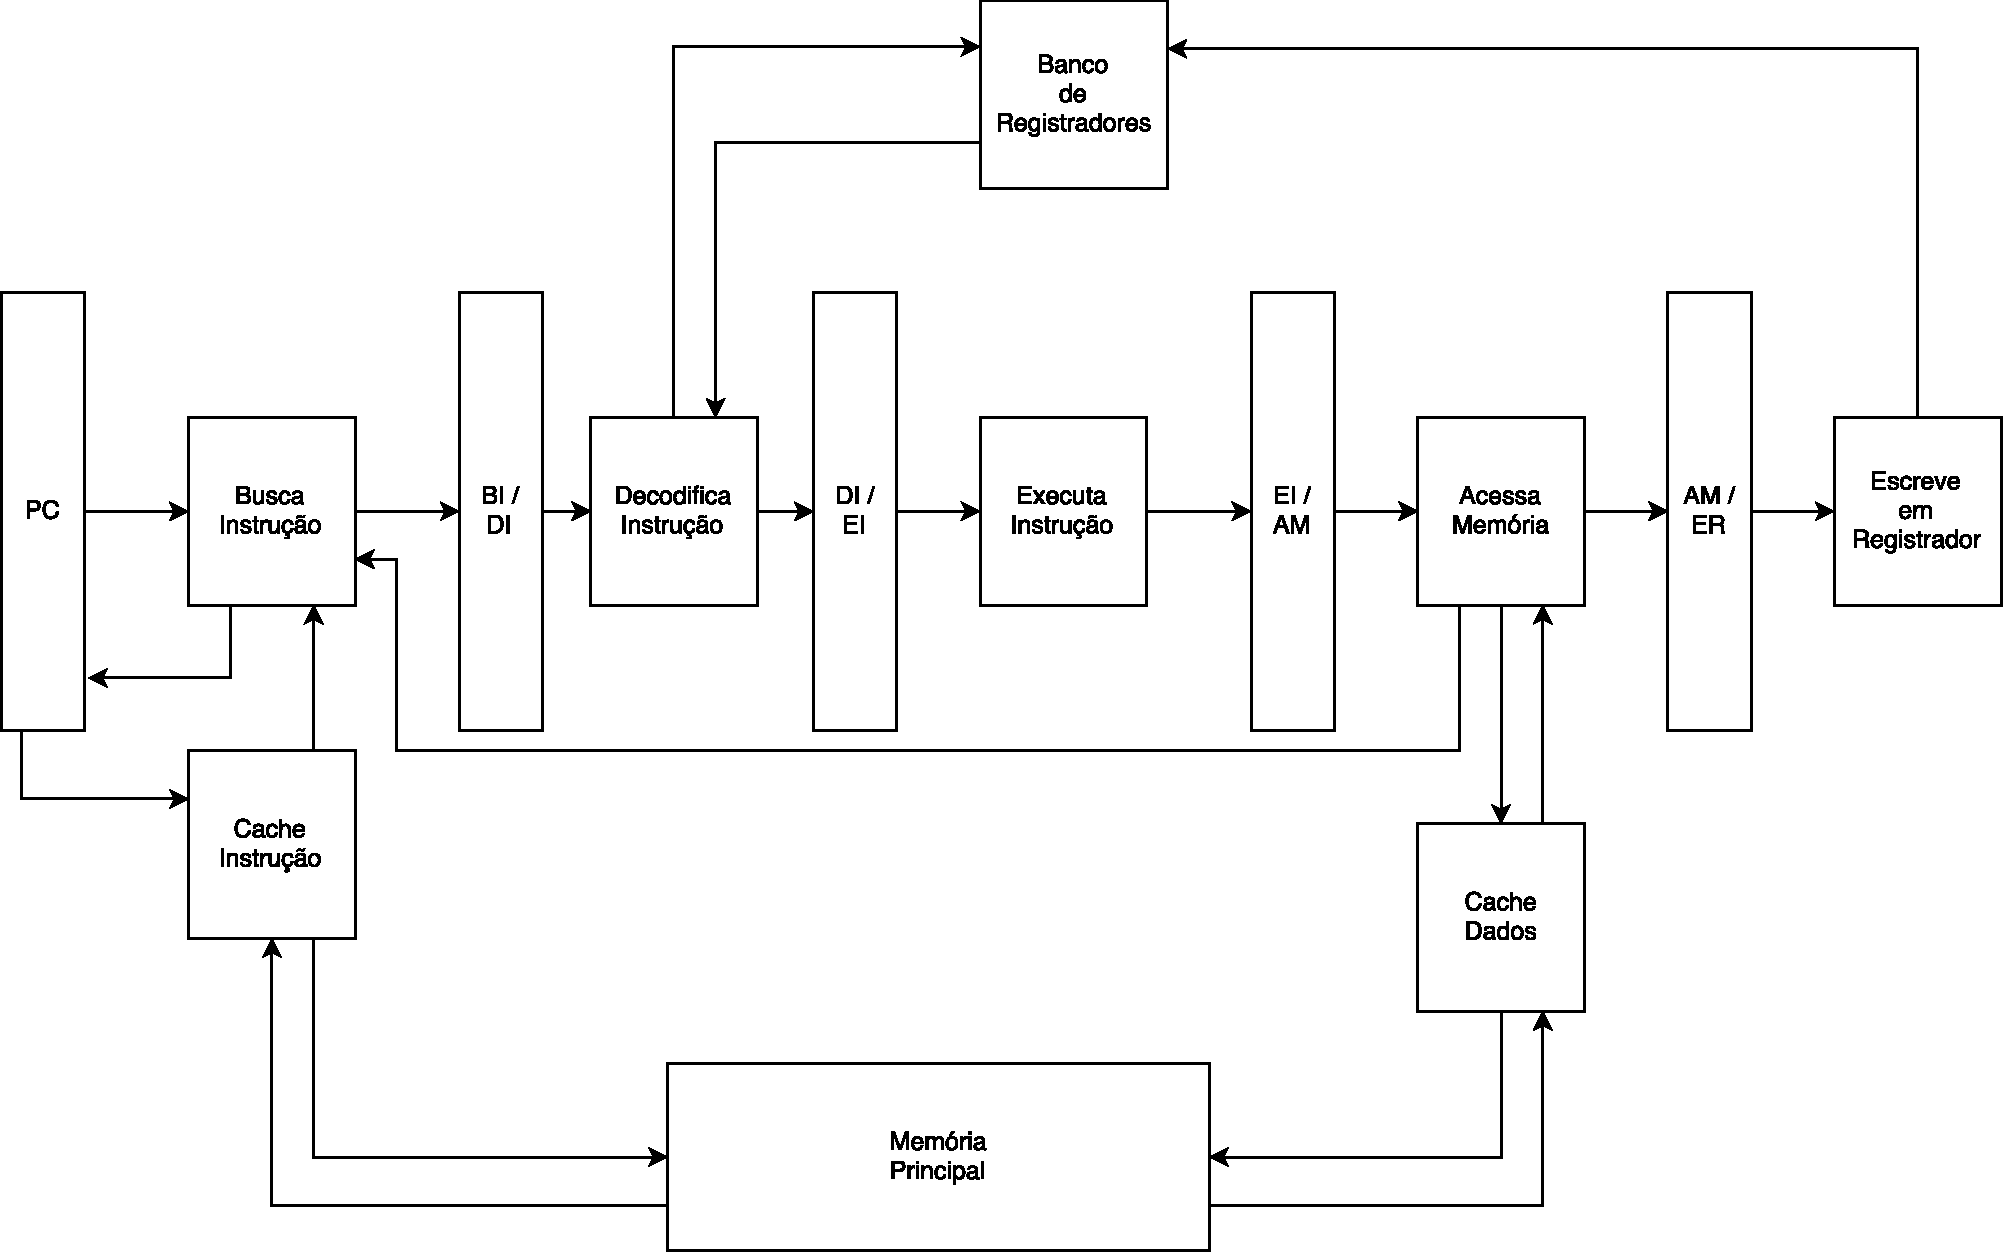
\includegraphics[scale=0.35, angle=0]{FEMTOMIPS_GLOBAL1}
    \caption{Os blocos básicos de uma implementação em pipeline da arquitetura do FEMTOMIPS}
	\end{figure}

	Uma versão idealizada dos blocos componentes da organização em pipeline do FEMTOMIPS é apresentada na \textbf{Figura 1}. 
	
	
	No diagrama: 
	
	\begin{itemize}
	\item \textbf{BI/DI, DI/EI, EI/AM, AM/ER} são registradores: PC armazena o endereço de leitura de comandos, enquanto que os demais armazenam o resultado de cada estágio do pipeline e o oferecem ao estágio seguinte. 
	\item \textbf{Busca Instrução, Decodifica Instrução, Executa Instrução, Acessa Memória, Escreve em Registrador} são blocos combinatórios que implement
	\item Os caches
	\end{itemize}
		
	

\subsubsection{A unidade de Forwarding}

	\begin{figure}[!ht]
  	\centering	
    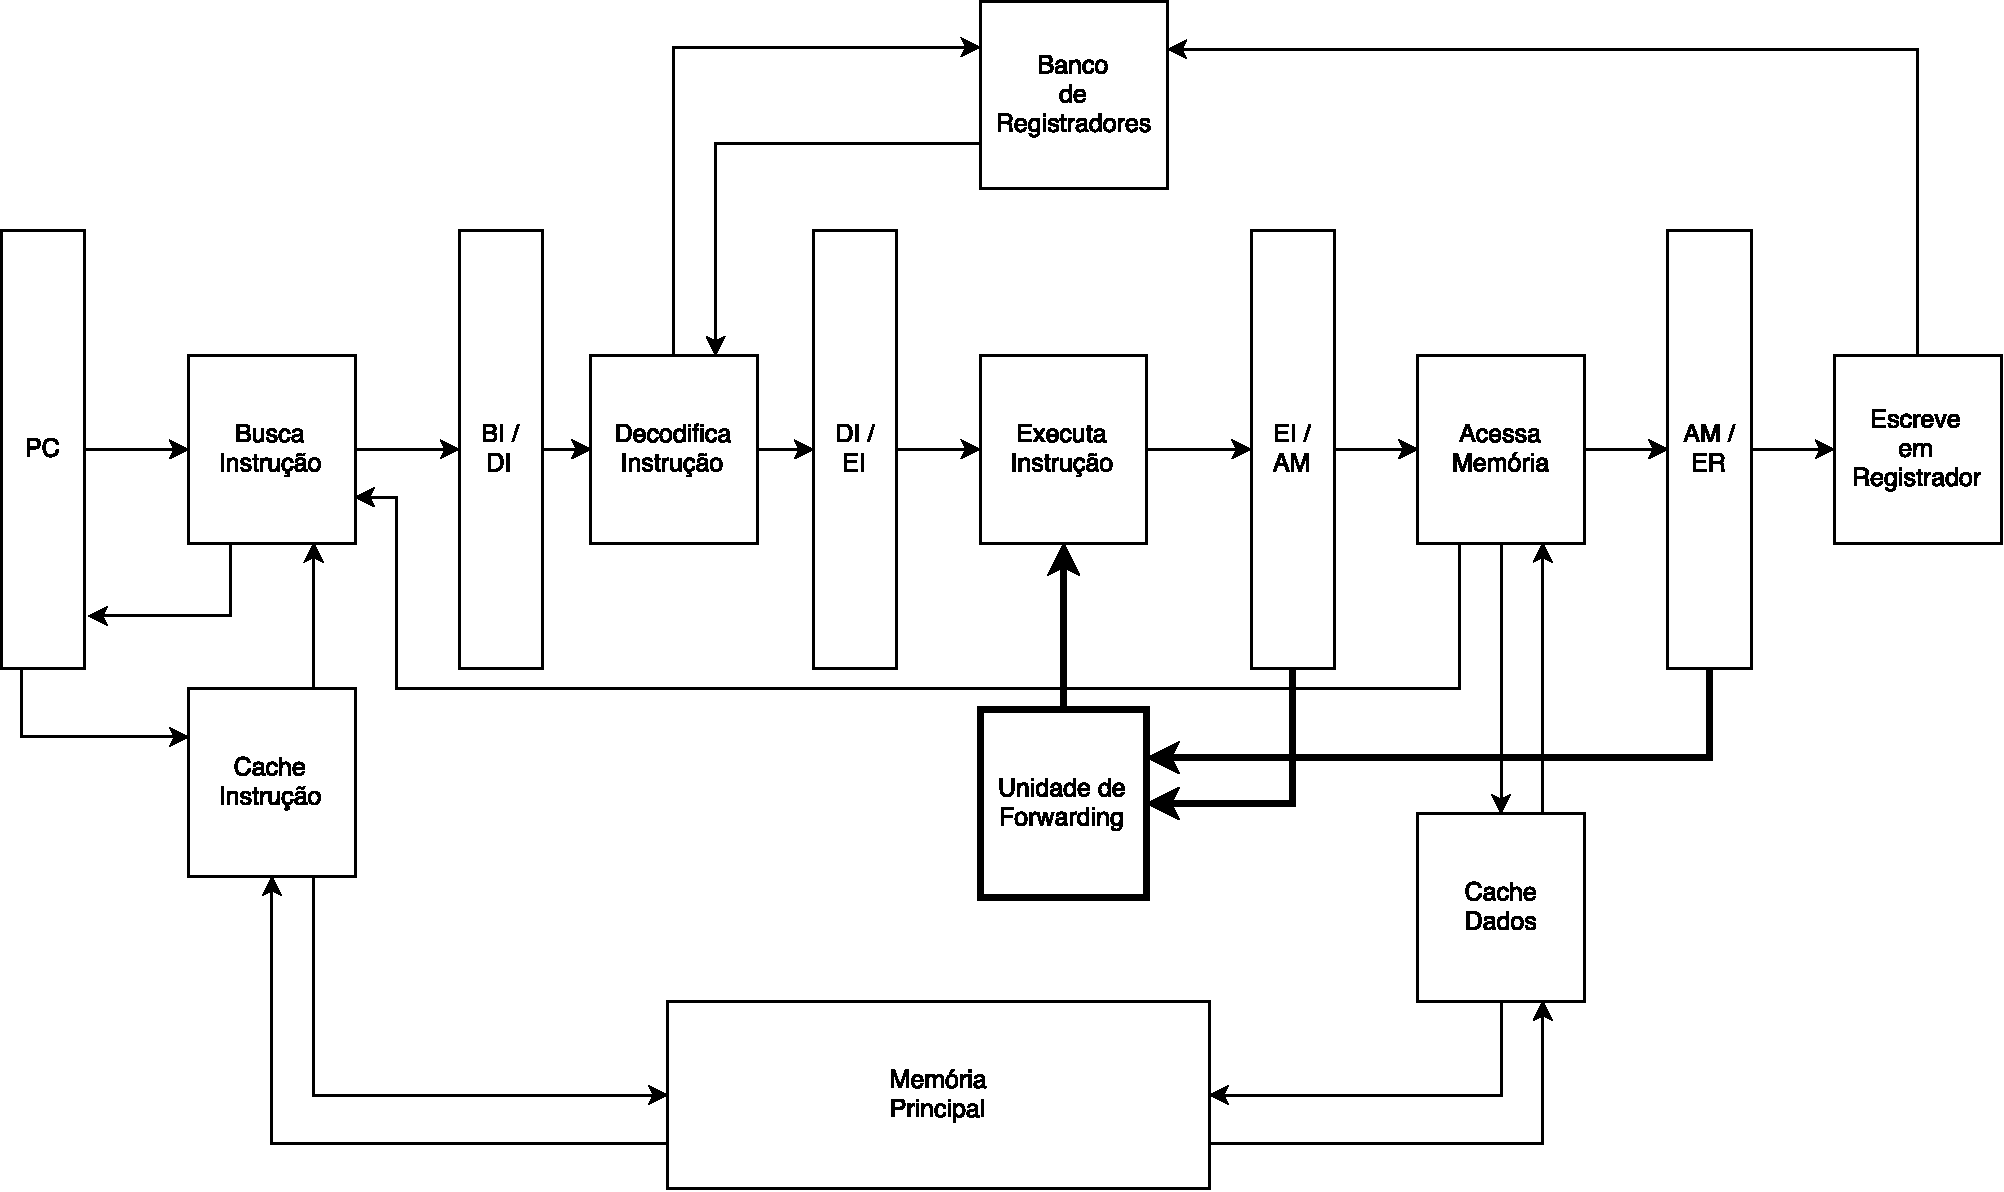
\includegraphics[scale=0.50, angle=270]{FEMTOMIPS_GLOBAL_FORWARDING}
    \caption{A unidade de Forwarding no contexto do FEMTOMIPS}
	\end{figure}

	
\subsubsection{Tratamento de Hazards de Dado}

	\begin{figure}[!ht]
  	\centering	
    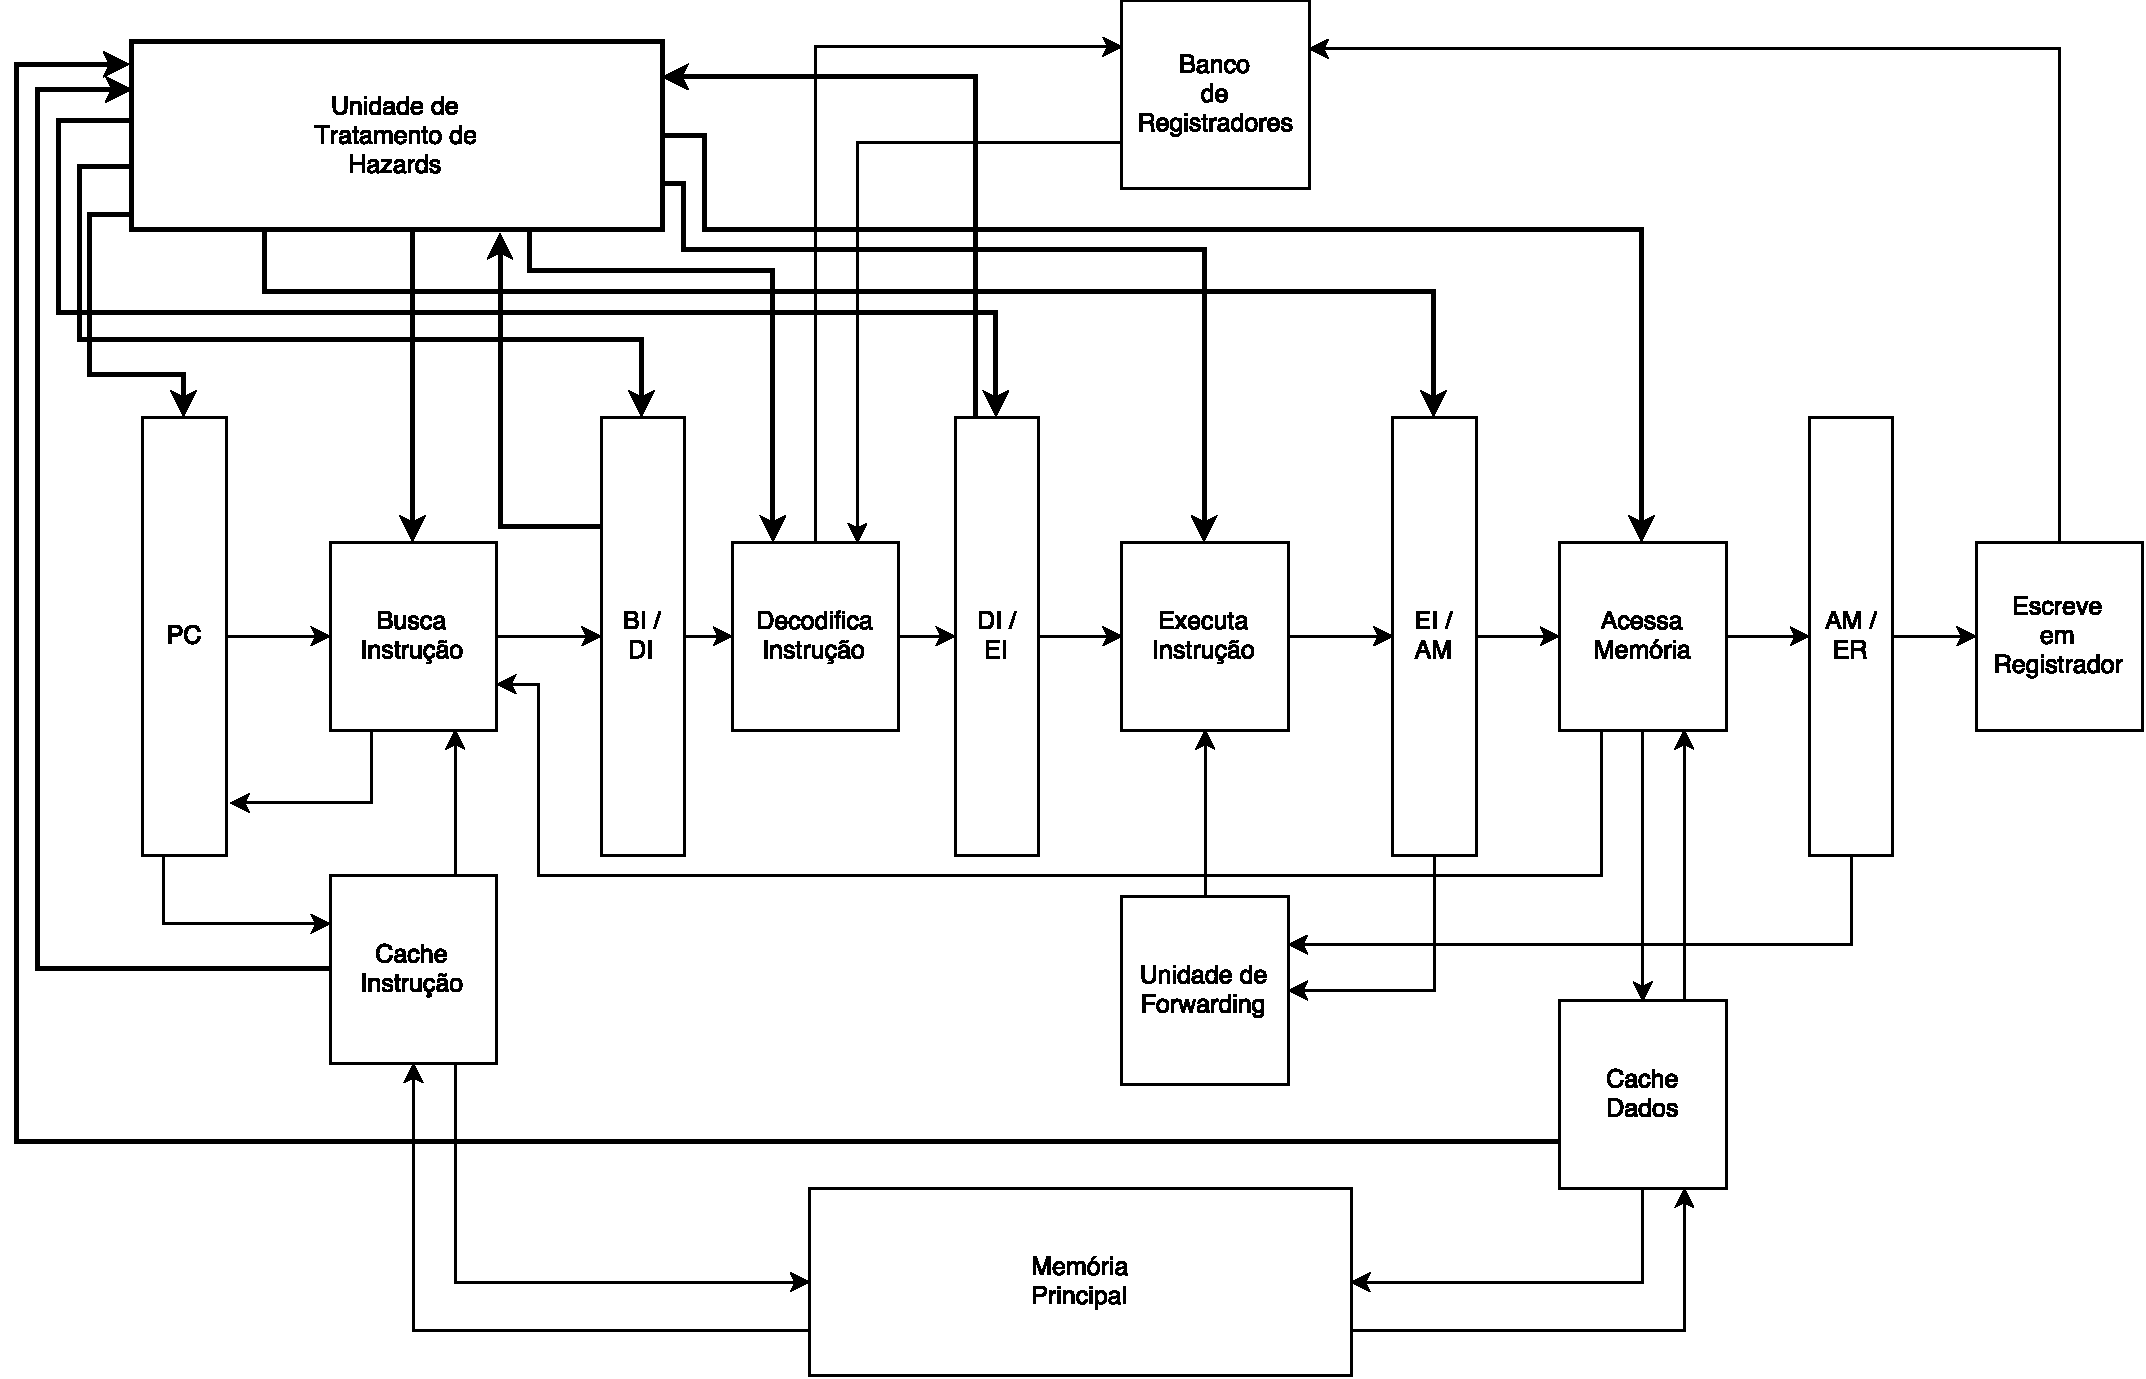
\includegraphics[scale=0.50, angle=270]{FEMTOMIPS_GLOBAL_HAZARDS}
    \caption{A unidade de Tratamento de Hazards no contexto do FEMTOMIPS}
	\end{figure}
	
\subsubsection{Tratamento de Hazards de Dado}

	\begin{figure}[!ht]
  	\centering	
    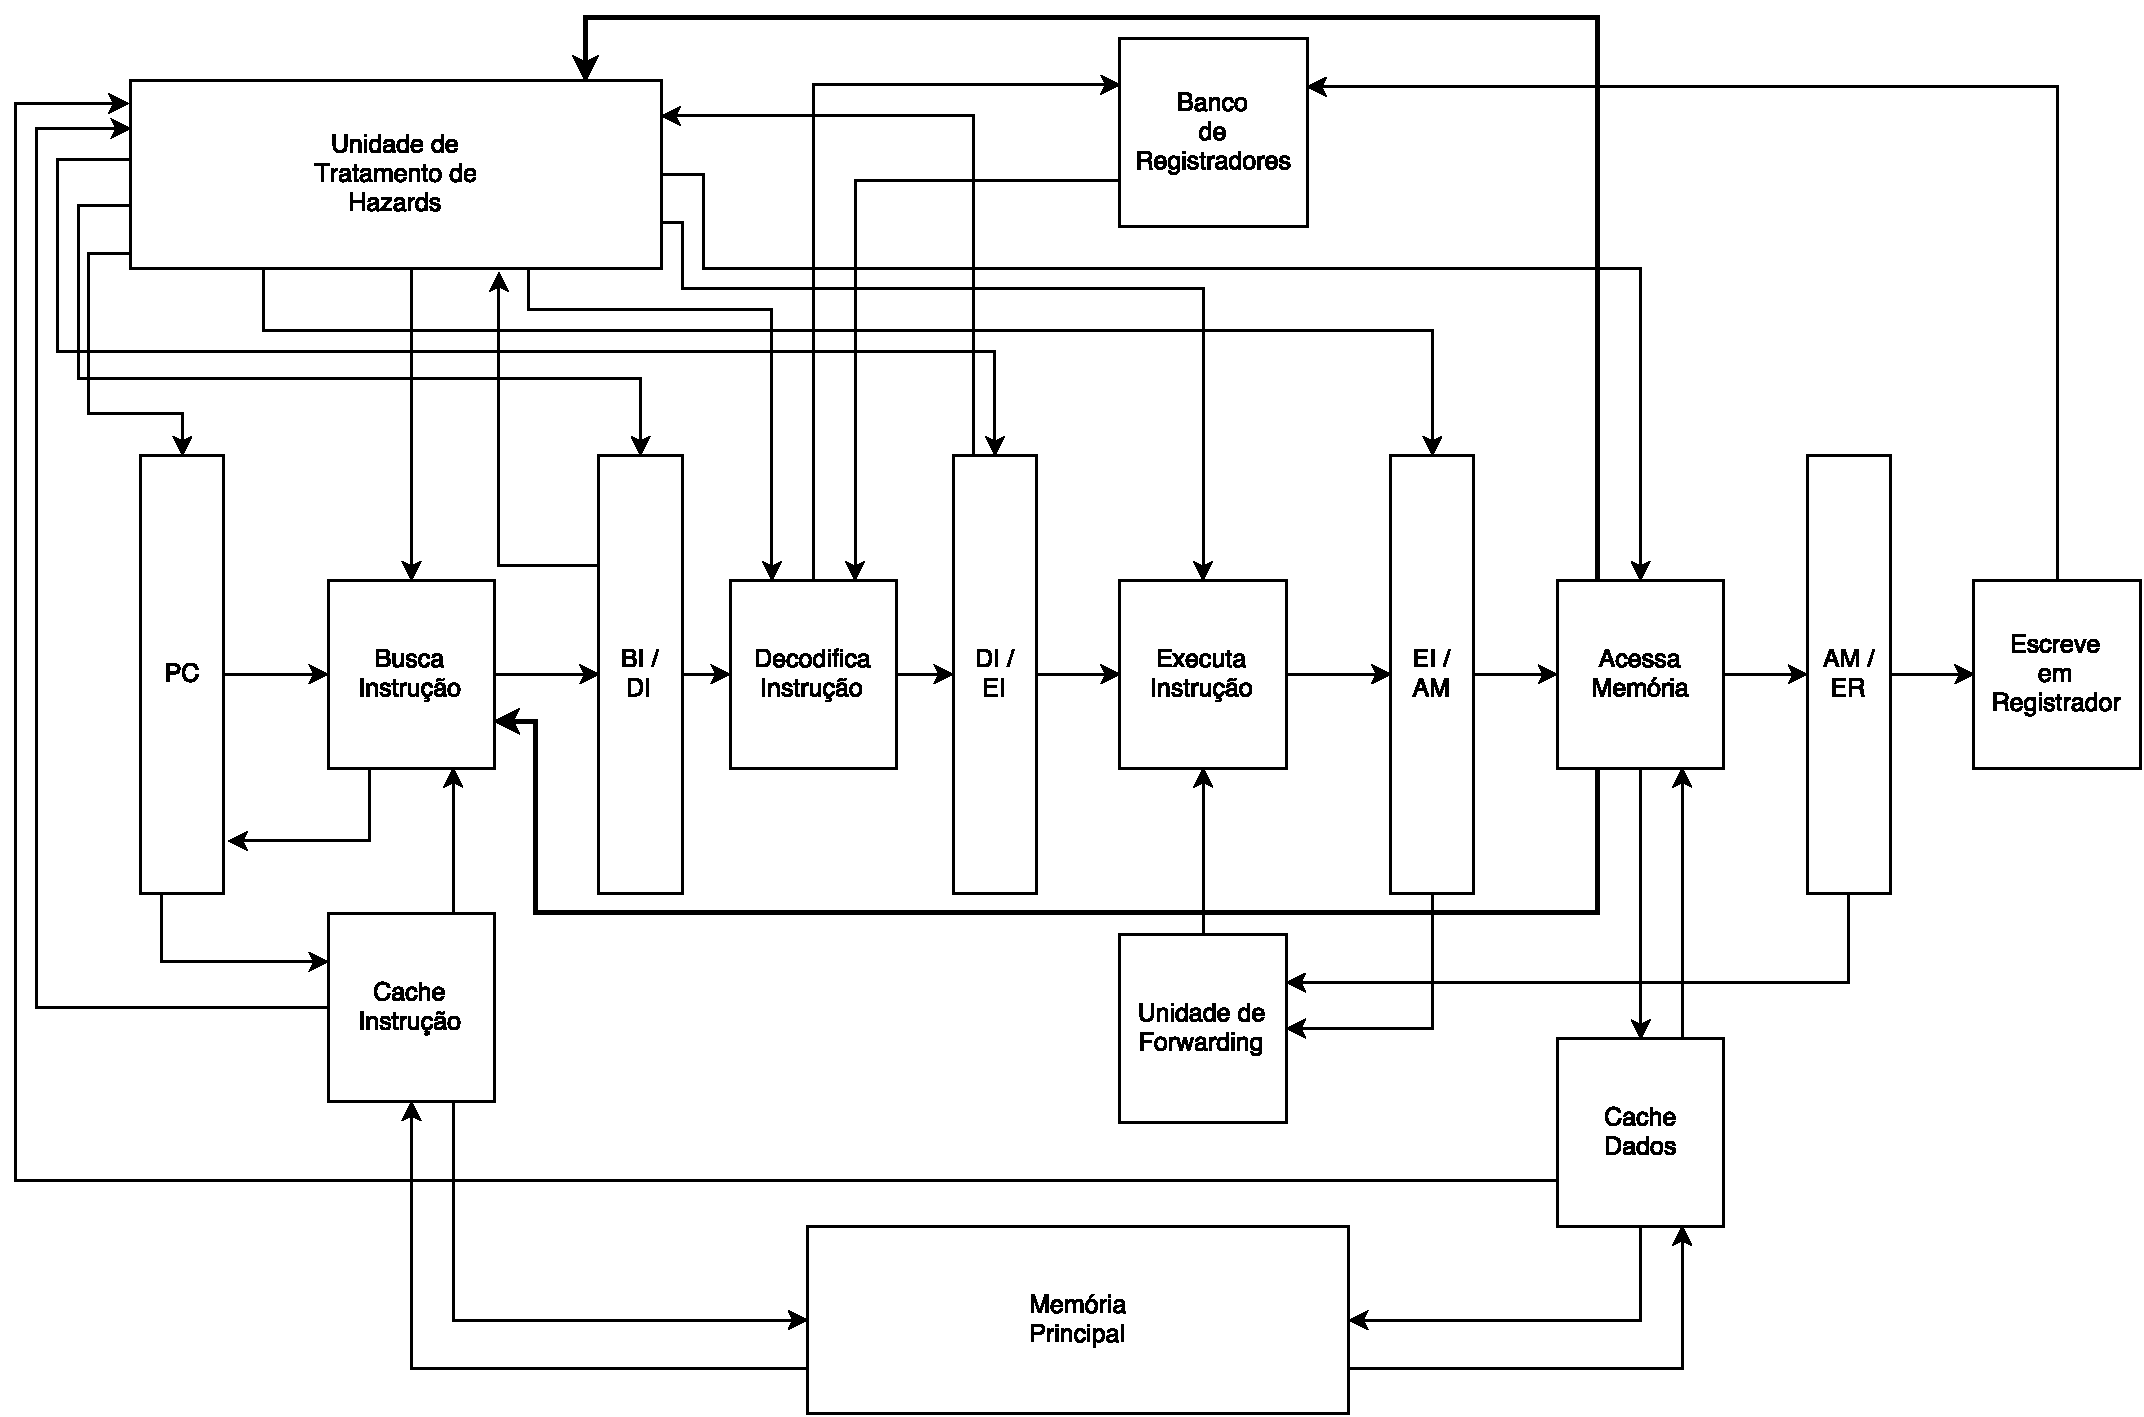
\includegraphics[scale=0.50, angle=270]{FEMTOMIPS_GLOBAL_BRANCH}
    \caption{Ligações adicionais para tratamento dos hazards de controle FEMTOMIPS}
	\end{figure}

\subsubsection{Lógica de interrupção}

	\begin{figure}[!ht]
  	\centering	
    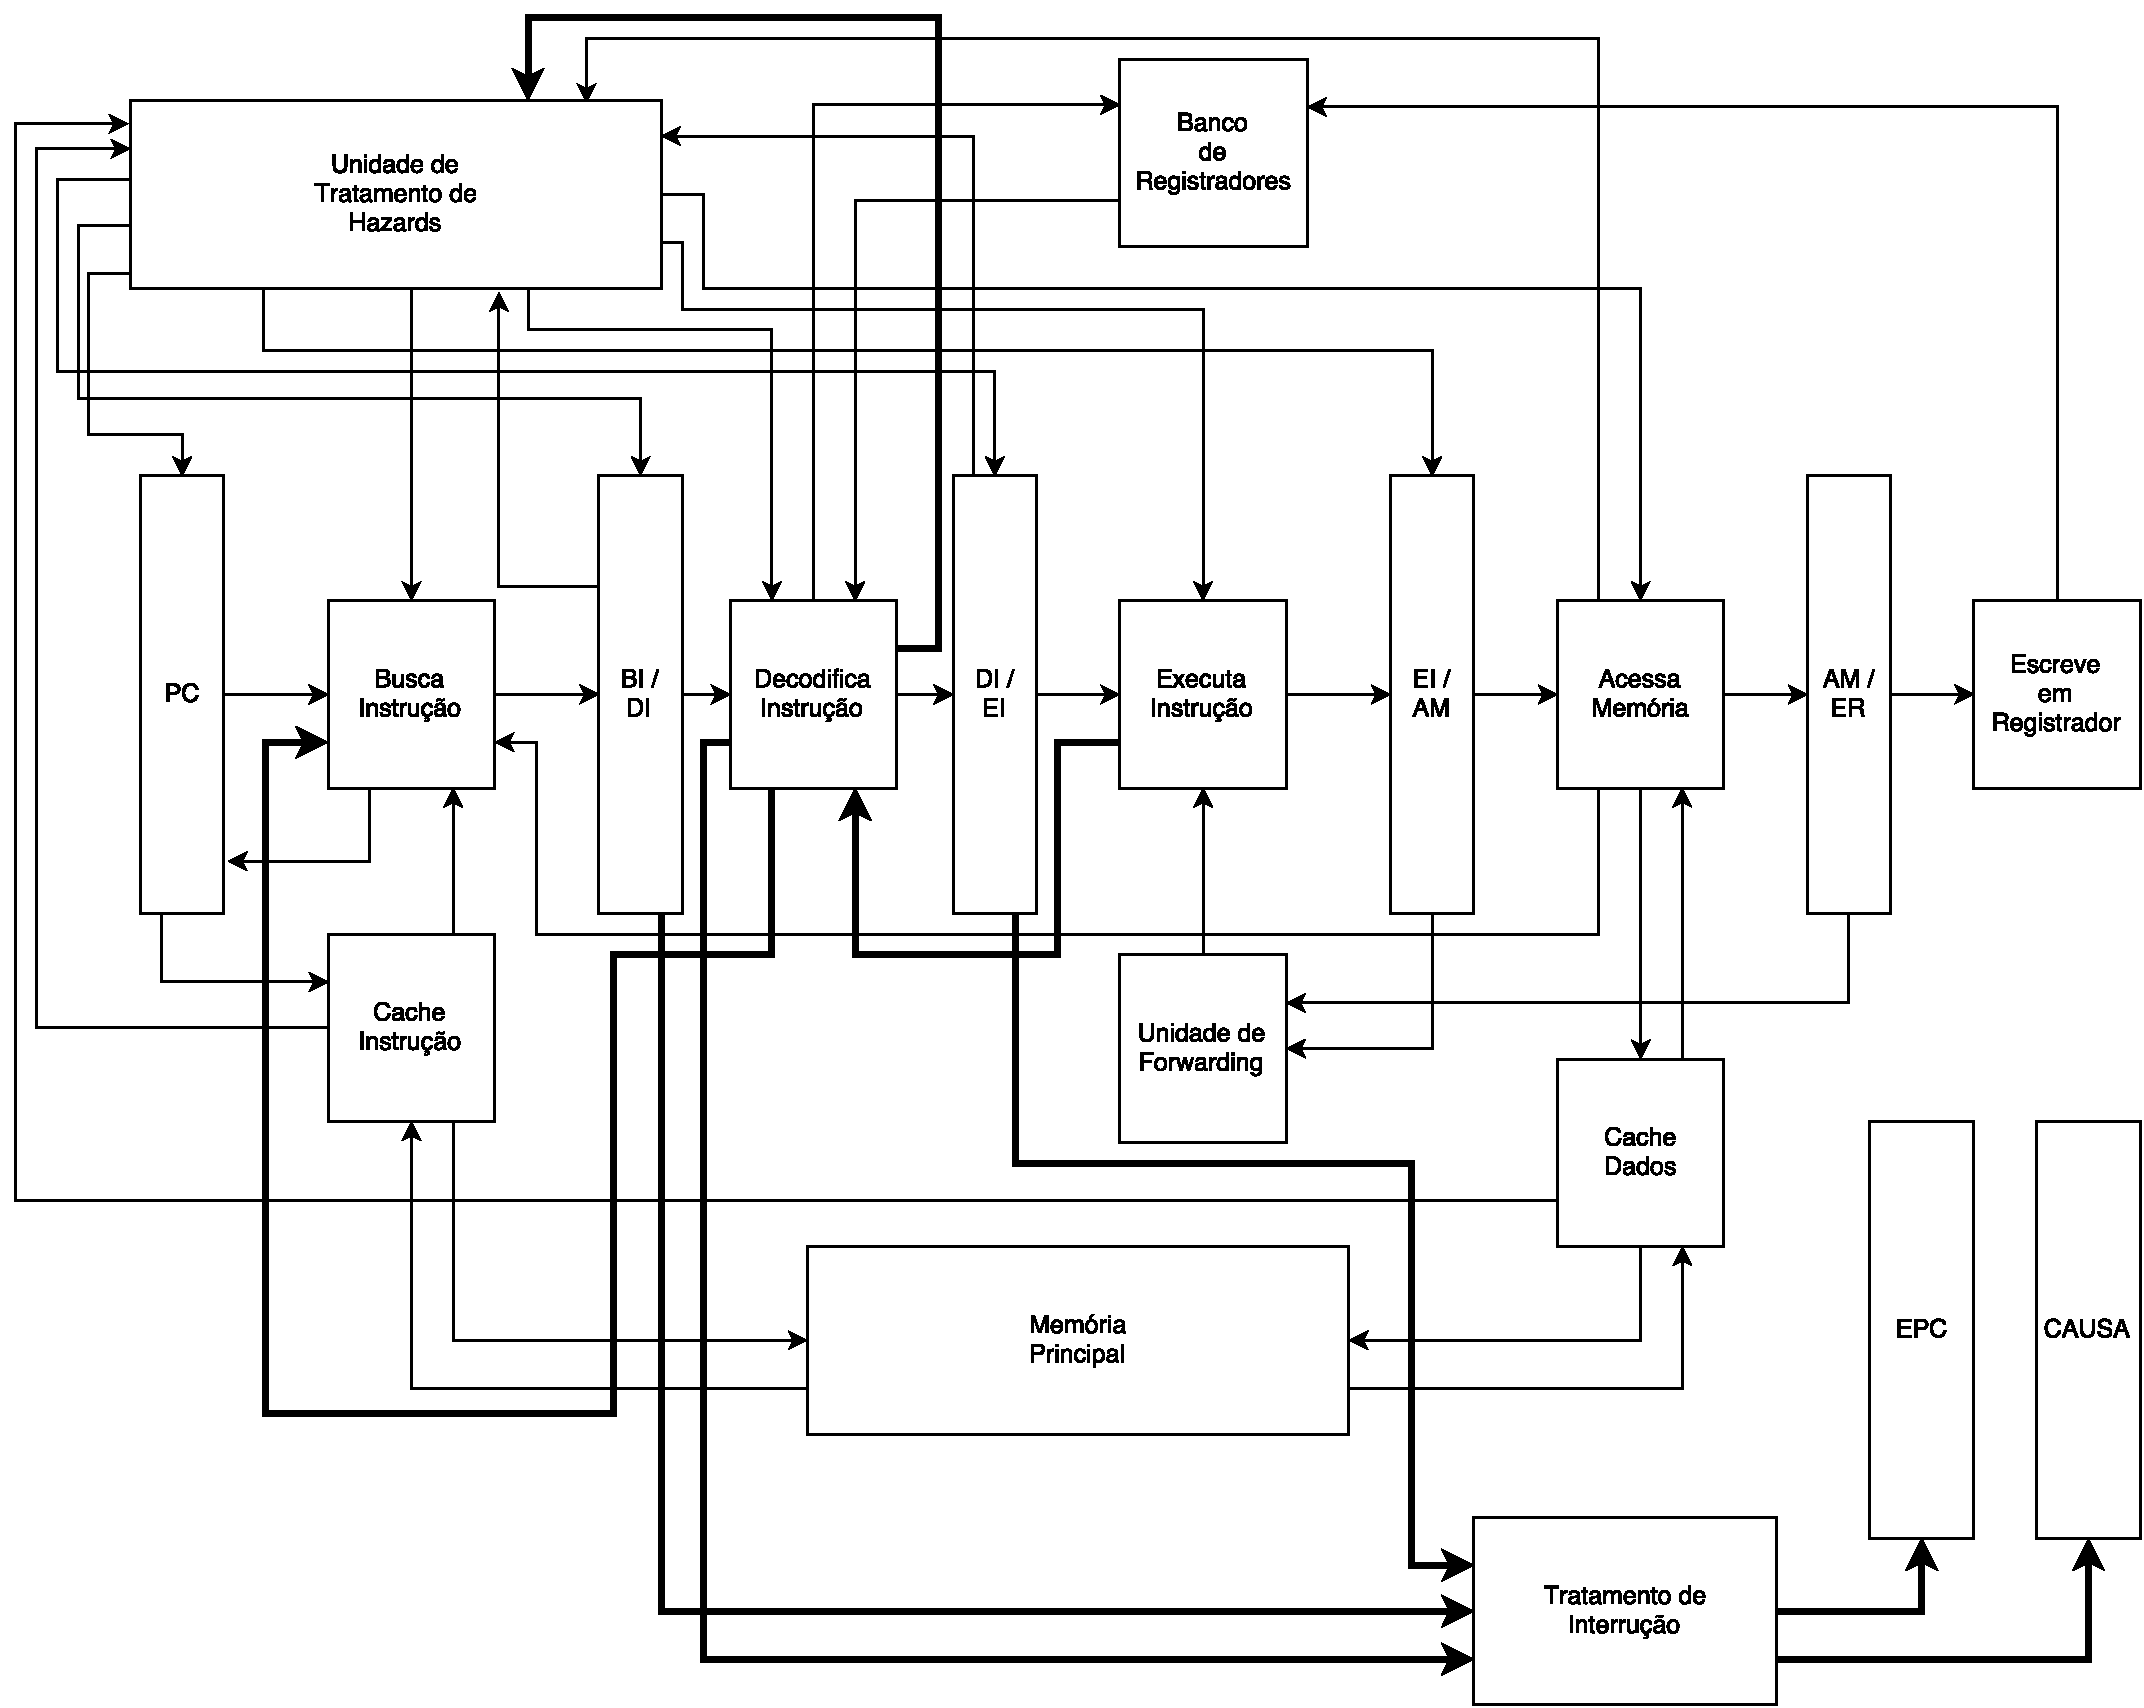
\includegraphics[scale=0.50, angle=270]{FEMTOMIPS_GLOBAL_INTERRUPT}
    \caption{O Tratamento de Interrupção no contexto do FEMTOMIPS}
	\end{figure}
	
\subsubsection{Lógica para simulação e coleta de dados}
	
	\begin{figure}[!ht]
  	\centering	
    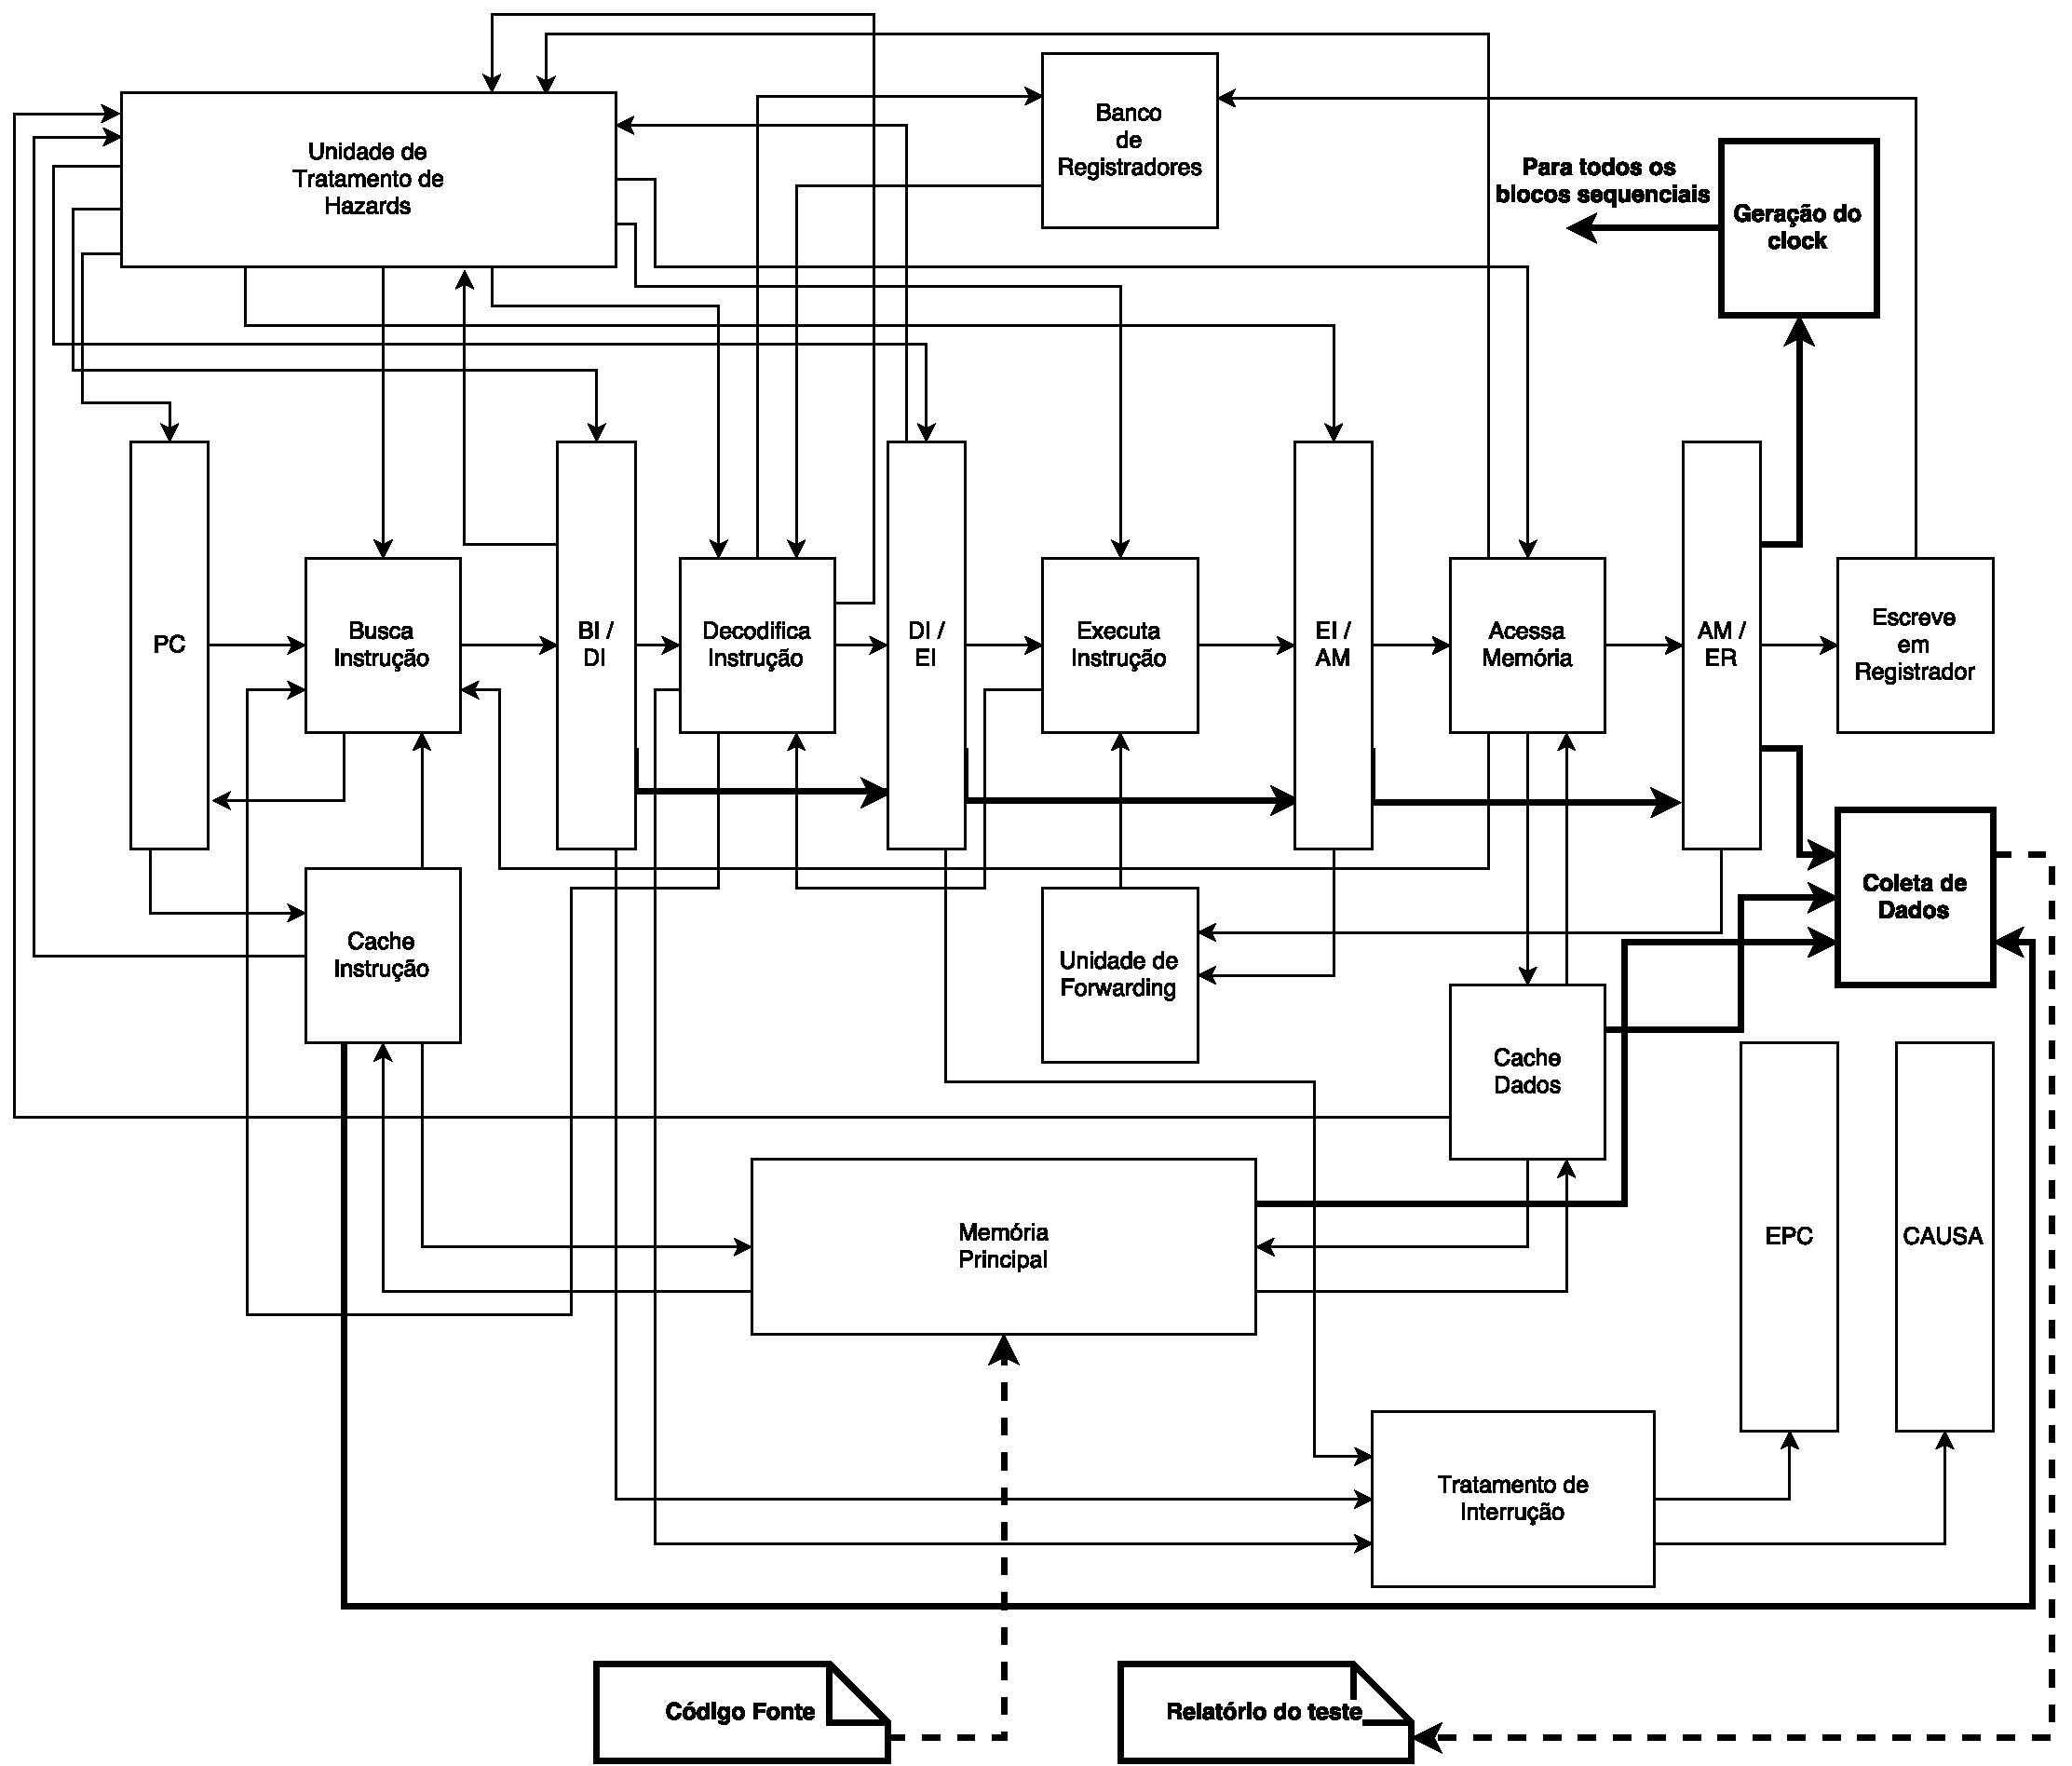
\includegraphics[scale=0.50, angle=270]{FEMTOMIPS_GLOBAL_MODELO}
    \caption{Estruturas adicionais para simulação e coleta de dados do FEMTOMIPS}
	\end{figure}

\end{document}